\documentclass[conference]{IEEEtran}
\IEEEoverridecommandlockouts
% The preceding line is only needed to identify funding in the first footnote. If that is unneeded, please comment it out.
\usepackage[T1]{fontenc}     % default is 'OT1'
%\usepackage[utf8]{inputenc} % needed if you have an older TeX distribution
\usepackage{lmodern}         % recommended
%\usepackage{citation}
\usepackage{amsmath,amssymb,amsfonts}
\DeclareMathOperator{\atan}{atan}
\DeclareMathOperator{\diag}{diag}
\usepackage{algorithmic}
\usepackage{graphicx}
\usepackage{textcomp}
\usepackage{xcolor}
\usepackage{tabularx}
\usepackage[hidelinks]{hyperref}
\usepackage{nicefrac}
\usepackage[inline]{enumitem}

\usepackage{acronyms}
\usepackage{todonotes}


% MUST BE LAST%
\usepackage[capitalise]{cleveref}

\begin{document}

\title{Paper title
\thanks{
    Funding info
}
}


\author{\IEEEauthorblockN{Ruslan Shaiakhmetov}
\IEEEauthorblockA{\textit{Department of Computer Science and Engineering} \\
\textit{Alma Mater Studiorum---Università di Bologna}\\
Cesena, Italy \\
0009-0001-0869-6204}
}


\maketitle

\begin{abstract}
Abstract goes here.

\end{abstract}

\begin{IEEEkeywords}
keyword1, keyword2, keyword3
\end{IEEEkeywords}

\section{Introduction}\label{sec:introduction}

Introduction goes here.

\paragraph{Problem statement}
Problem statement goes here.

\paragraph{Contribution}
Contribution goes here.

\section{Related Work}
\label{sec:state-of-the-art}

Related work goes here.
\section{Proposed approach}
\label{sec:proposed-approach}

Proposed approach goes here.

\section{Experimental evaluation}
\label{sec:experimental-evaluation}

\begin{figure}
    \begin{center}
        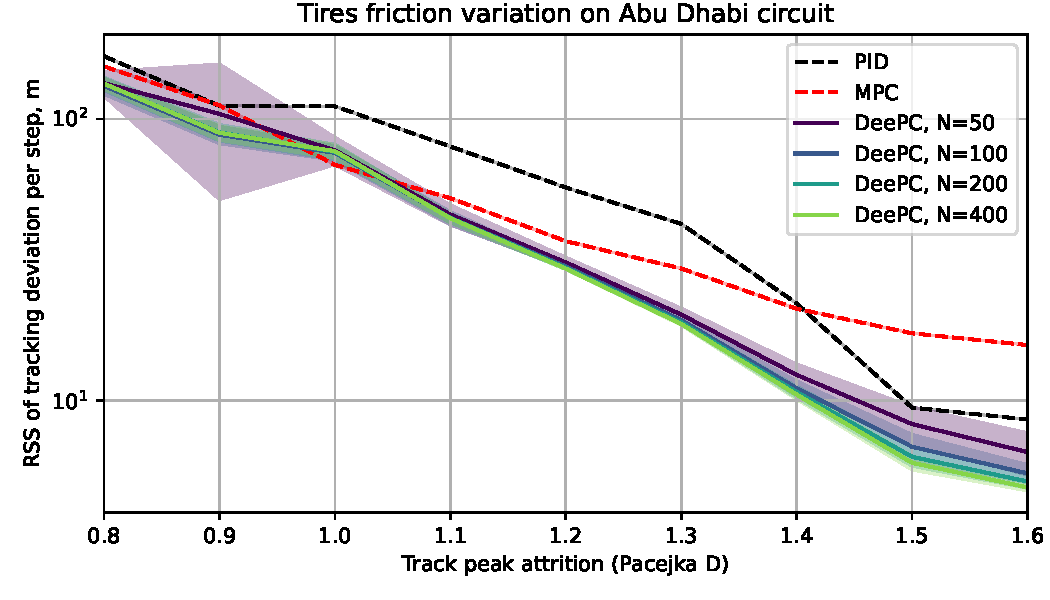
\includegraphics[width=0.47\textwidth]{img/Abu_Dhabi_new.pdf}
        \caption[Tires friction variation on Abu Dhabi circuit]{
            Error with increasingly higher peak tyre friction in the Yas Marina circuit.
            \ac{deepc} outperforms both the baselines.
            Solid lines are averaged over 30 repetitions,
            colored shades areas depict $\pm$ one standard deviation.
        }
        \label{fig:realtrack}
    \end{center}
\end{figure}

Experimental evaluation goes here.

\section{Conclusion and future work}
\label{sec:conclusions}

Conclusion and future work goes here.

\bibliographystyle{IEEEtran}
\bibliography{bibliography}

\vspace{12pt}

\end{document}
